\documentclass[tikz,border=10pt]{standalone}\begin{document}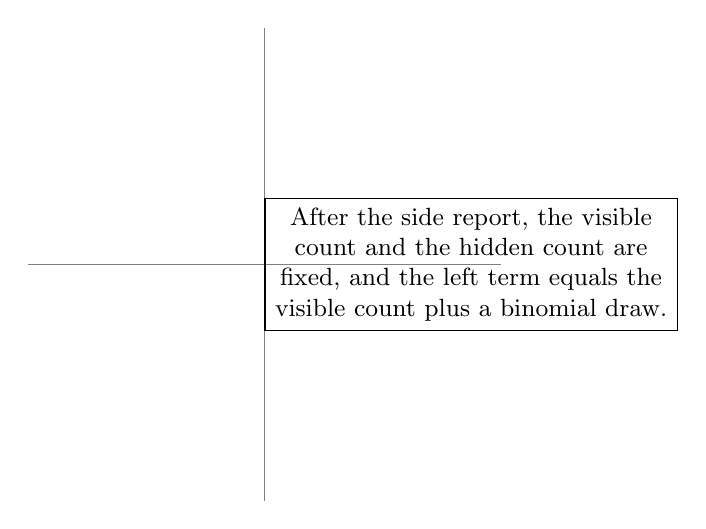
\begin{tikzpicture}[x=1cm,y=1cm]\draw[gray] (0,0) -- (6,0);\draw[gray] (3,-3) -- (3,3);\node[draw, text width=5cm, align=center, font=\small, anchor=west] at (3, 0) {After the side report, the visible count and the hidden count are fixed, and the left term equals the visible count plus a binomial draw.};\end{tikzpicture}\end{document}\n